\documentclass[12pt, a4paper]{article}
\usepackage{float}
\usepackage[utf8]{inputenc}
\usepackage[T1]{fontenc}
\usepackage{newtxtext,newtxmath} % Times New Roman equivalent font in LaTeX
\usepackage[top=2cm, bottom=2.5cm, left=3cm, right=1.5cm]{geometry}
\usepackage{graphicx}
\usepackage{amsmath}
\usepackage{booktabs}
\usepackage{indentfirst}
\usepackage{caption}
\usepackage{hyperref}

% Page and document settings to match AITU template specifications
\setlength{\parindent}{1.25cm}
\renewcommand{\baselinestretch}{1.0}
\captionsetup[figure]{font=small,labelfont=bf,justification=centering,name={Fig.}}
\captionsetup[table]{font=small,labelfont=bf,position=top,justification=justified}

% Ensure section headers match standard formatting style
\usepackage{titlesec}
\titleformat{\section}{\normalfont\fontsize{12}{14}\bfseries}{\thesection}{1em}{}
\titleformat{\subsection}{\normalfont\fontsize{12}{14}\itshape}{\thesubsection}{1em}{}

\title{TASK-AWARE ANALYSIS OF JPEG RECOMPRESSION AND BIT-DEPTH REDUCTION FOR OBJECT DETECTION}

\author{
  \textbf{Amir Karataev} \\
  \small Master of Science, Graduate Student, Department of Computer Engineering \\
  \small amir.karataev@example.com, ORCID: 0000-0002-XXXX-XXXX \\
  \small Astana IT University, Kazakhstan
}
\date{}

\begin{document}

\maketitle

\begin{abstract}
This paper presents a task-aware empirical investigation into the effects of image compression and quantization on downstream deep learning-based computer vision systems. Traditional image compression frameworks have historically been optimized for visual appeal to human observers, using perceptual metrics such as Peak Signal-to-Noise Ratio (PSNR) and Structural Similarity Index Measure (SSIM). However, modern autonomous workflows increasingly rely on neural networks, whose feature-extraction pipelines process visual artifacts differently than the human visual system. To bridge this research gap, we evaluate two distinct image degradation and storage strategies using the standard COCO val2017 dataset (5,000 images) and a YOLOv8n object detection model. The first branch utilizes JPEG recompression at quality levels 94, 88, 75, 50, and 25. The second branch applies uniform RGB bit-depth reduction (BPC) to 7, 4, 3, 2, and 1 bits per channel, stored in a lossless PNG container. Our findings reveal a significant divergence between classical visual quality and downstream task performance. JPEG recompression exhibits remarkable efficiency; quality level 88 achieves 2.02$\times$ storage reduction (halving the dataset size to 384.22 MB) with a negligible relative drop in mean Average Precision (mAP50) of less than 1\% (0.5147 compared to the baseline 0.5187). Conversely, the uniform bit-depth reduction branch yields poor storage-task efficiency when constrained by the PNG container. While 7-bit quantization preserves baseline object detection performance (0.5189 mAP50), its file size inflates to 1912.67 MB (0.41$\times$ negative compression) due to spatial banding ruining the entropy coding efficiency of the PNG DEFLATE algorithm. Furthermore, BPC levels that achieve storage savings ($b \le 3$) cause a catastrophic drop in detection accuracy ($>15.3\%$ drop at $b=3$, and near total failure at lower bitrates). We conclude that under the evaluated BPC + PNG storage scheme, JPEG recompression is vastly more efficient for task-aware machine vision workflows, and we establish that visual quality metrics alone are insufficient predictors of deep learning task stability.
\end{abstract}

\noindent \textbf{Keywords:} Image Compression; Quantization; JPEG Recompression; Bit-Depth Reduction; Object Detection; YOLOv8; COCO Dataset; PSNR; SSIM; mAP.

\section{Introduction}
With the rapid proliferation of the Internet of Things (IoT), autonomous vehicles, remote sensing, and urban video surveillance, vast quantities of visual data are generated and processed continuously. Traditionally, digital image pipelines have been engineered with the human observer in mind. In these legacy systems, raw sensor arrays are subjected to lossy compression algorithms designed to eliminate visual redundancies that are imperceptible to human eyes, thereby minimizing storage and transmission bandwidth while maximizing visual comfort. 

However, a fundamental paradigm shift is currently underway. An increasing majority of digital images are no longer inspected by human eyes; instead, they are ingested directly by convolutional neural networks (CNNs) and vision transformers executing automated downstream tasks such as object detection, semantic segmentation, and instance tracking. This shift exposes a critical mismatch: the mathematical features and spatial patterns prioritized by deep networks during backpropagation do not necessarily align with the perceptual criteria of human biological vision.

Standard image quality assessment (IQA) metrics, such as Peak Signal-to-Noise Ratio (PSNR) and Structural Similarity Index Measure (SSIM), operate under the assumption that spatial fidelity and error visibility are the ultimate measures of image utility. Yet, deep networks process images through layers of mathematical filters that extract abstract edges, high-frequency contours, and color gradients. Consequently, an image that appears blocky or heavily quantized to a human observer might still preserve the structural features necessary for a neural network to produce high-confidence bounding boxes. Conversely, subtle high-frequency smoothing or color shifts that are visually imperceptible to humans can disrupt the internal activations of a deep model, leading to classification errors or missed detections.

This problem is particularly relevant for systems operating under constrained resources: mobile devices, edge-AI platforms, autonomous cameras, unmanned aerial vehicles, and embedded solutions, where it is necessary to simultaneously reduce the volume of transmitted or stored data while preserving the suitability of images for automated analysis. Therefore, investigating image compression with respect to the downstream task of object detection is a timely concern from both scientific and practical perspectives.

This study investigates the practical trade-off between dataset storage size and downstream task accuracy. Specifically, we conduct a controlled empirical comparison of two distinct image degradation mechanisms:
\begin{enumerate}
    \item \textbf{JPEG Recompression}: A frequency-domain lossy compression scheme. It applies discrete cosine transform (DCT) blocks and quantizes high-frequency coefficients, yielding substantial storage savings but introducing blocky artifacts and ringing around high-contrast boundaries.
    \item \textbf{Bit-Depth Reduction (BPC)}: An amplitude-domain quantization scheme. It reduces the number of bits allocated to each color channel (from the standard 8-bit representation down to 1-bit), stored inside a lossless Portable Network Graphics (PNG) container. This preserves sharp geometric boundaries but limits amplitude resolution, introducing color banding and artificial contours.
\end{enumerate}

By evaluating these pipelines using the state-of-the-art YOLOv8n detector on the Microsoft COCO val2017 dataset, we address a key research question: \textit{When constrained to a fixed storage budget, which degradation mechanism preserves downstream object detection accuracy more effectively?}

Our working hypothesis is that the sensitivity of an object detection model is determined not only by the degree of information loss, but also by the nature of the distortions introduced. Consequently, JPEG compression and bit-depth reduction, even at comparable levels of compression, may affect detection quality in fundamentally different ways.

The scientific novelty of this work lies in the comparative investigation of two distinct mechanisms of image information loss---frequency-domain JPEG quantization and amplitude-domain bit-depth reduction---evaluated not only by their effects on visual image characteristics, but also by their impact on the downstream task of object detection. Unlike traditional approaches, which assess compression quality primarily through visual fidelity metrics, this study simultaneously evaluates compression efficiency across file size metrics, classical distortion metrics, and application-level object detection metrics.

The practical significance of the results extends to the design of visual data pipelines for edge-AI cameras, drones, mobile computer vision systems, video surveillance networks, image transmission channels for automated analysis, and low-resource embedded platforms. Specifically, this work provides empirically grounded guidance on which compression regimes are acceptable and which types of distortions are most detrimental to neural network-based object detection.

Ultimately, this work presents a task-aware evaluation framework that challenges the reliance on visual similarity metrics for machine-centric visual pipelines. We demonstrate that JPEG recompression provides a highly efficient and gradual trade-off curve, whereas uniform BPC stored via PNG suffers from severe container-level storage inflation and rapid detection degradation at lower bit depths.

\section{Literature Review}
The intersection of digital image compression, visual quality evaluation, and deep learning-based computer vision has attracted significant academic interest. This section reviews the historical development and current state of research in these domains.

\subsection{Classical Image Compression and Coding Standards}
The evolution of classical image compression standards relies heavily on exploiting spatial and statistical redundancies. The Joint Photographic Experts Group (JPEG) standard, formalized by Wallace \cite{wallace1992}, remains the most widely deployed lossy compression framework. JPEG operates in the frequency domain, partitioning the image into $8\times8$ pixel blocks, applying a Discrete Cosine Transform (DCT), and quantizing the resulting coefficients based on a human visual sensitivity matrix. While highly effective at low to medium compression ratios, JPEG's block-based nature introduces prominent blocking artifacts and high-frequency noise at low quality factors.

In contrast, the Portable Network Graphics (PNG) format, specified by the World Wide Web Consortium \cite{w3c2003}, represents the standard for lossless spatial-domain storage. PNG utilizes a two-stage compression pipeline consisting of spatial prediction filtering followed by DEFLATE entropy coding. While lossless PNG preserves exact pixel-level fidelity, its compression efficiency depends heavily on the presence of smooth, repetitive spatial patterns and low-frequency gradients. When images contain high-frequency noise or sharp transitions, PNG's spatial prediction models fail, leading to drastically reduced compression ratios.

\subsection{Image Quality Assessment}
For decades, IQA has relied on full-reference metrics such as PSNR and SSIM. PSNR computes the logarithmic ratio between the maximum possible power of a signal and the corrupting noise affecting its fidelity. However, PSNR is a purely pixel-difference metric that fails to account for human structural perception. To resolve this, Wang et al. \cite{wang2004} introduced the Structural Similarity Index Measure (SSIM), which models image degradation as a combination of luminance, contrast, and structural changes. While SSIM represents a significant advancement toward simulating human visual judgment, comparative studies by Horé and Ziou \cite{hore2010} demonstrate that PSNR and SSIM often exhibit non-linear behavior under different types of noise and distortions. As surveyed by Zhai and Min \cite{zhai2020}, traditional IQA metrics remain fundamentally human-centric. They are mathematically ill-suited for evaluating ``machine visual quality,'' as deep neural networks operate on statistical distributions and abstract semantic features rather than biological visual pathways.

\subsection{Color and Network Quantization}
Quantization represents the mathematical mapping of a continuous or high-precision set of values to a discrete, lower-precision representation. In computer graphics, Heckbert \cite{heckbert1982} pioneered spatial partitioning techniques, such as the median cut algorithm, to perform color image quantization for restricted frame buffers. To mitigate the visual banding caused by severe color depth reduction, Floyd and Steinberg \cite{floyd1976} developed error-diffusion dithering, which scatters quantization errors across neighboring pixels. While dithering improves human visual appeal by simulating continuous tones, it introduces massive high-frequency spatial noise, which can be highly disruptive to CNN feature extraction.

Parallel to image-level quantization, deep learning researchers have extensively explored network-level quantization. Jacob et al. \cite{jacob2018} demonstrated that quantizing network weights and activations to 8-bit integer formats enables efficient inference on edge hardware with minimal loss in accuracy. Similarly, Han et al. \cite{han2016} proposed ``Deep Compression,'' which integrates weight pruning, trained quantization, and Huffman coding to drastically compress deep neural network footprints. These efforts, however, focus on model weights rather than input image signals, leaving a significant gap in understanding how input-level color quantization interacts with standard networks.

\subsection{Deep Learning-Based Object Detection}
Object detection is a cornerstone of modern computer vision. Redmon et al. \cite{redmon2016} revolutionized this field by introducing the You Only Look Once (YOLO) framework, which formulated object detection as a single regression problem, enabling real-time inference. Over the past decade, the YOLO architecture has undergone numerous iterations to optimize speed and accuracy. Wang et al. \cite{wang2023} introduced YOLOv7, optimizing bag-of-freebies learning strategies and architectural scaling. The state-of-the-art YOLOv8 architecture, developed by Jocher et al. \cite{jocher2023}, incorporates an anchor-free split head and advanced spatial attention mechanisms, providing highly robust feature extraction across varying spatial resolutions. These models are typically trained and validated on complex datasets like Microsoft COCO, compiled by Lin et al. \cite{lin2014}, which contains 118,000 training and 5,000 validation images spanning 80 object categories.

\subsection{Task-Aware and Machine-Centric Compression}
With deep networks increasingly acting as the primary consumers of digital images, researchers have begun exploring ``compression for machines'' (CFM). Hu et al. \cite{hu2018} proposed a task-aware image compression pipeline tailored for cloud-based object detection, demonstrating that localized image patches containing target objects should be compressed with higher fidelity than background regions. Similarly, Kim et al. \cite{kim2021} developed a spatially-adaptive feature transform network that optimizes image compression directly against a machine vision objective function. Ye et al. \cite{ye2023} introduced AccelIR, demonstrating that joint optimization of image restoration and neural compression can accelerate downstream restoration tasks.

The impact of classical compression on deep networks remains a vital area of study. Gandor and Nalepa \cite{gandor2022} conducted systematic trials demonstrating that object detectors show non-linear sensitivity to JPEG compression, maintaining stable accuracy until a critical threshold is crossed, after which performance collapses. Hao et al. \cite{hao2022} extended this analysis by showing that image degradation interacts strongly with the physical size and distance of target objects, with smaller objects showing extreme sensitivity to compression noise. Modern surveys by Huang and Wu \cite{huang2024} and Piran \cite{piran2022} emphasize that developing end-to-end learned image compression standards for both human and machine eyes remains one of the most prominent challenges in contemporary computer vision.

\section{Methods and Materials}
To evaluate the effects of image degradation on downstream object detection, we built a highly rigorous and reproducible empirical pipeline. This section details the datasets, neural architectures, degradation algorithms, and evaluation metrics utilized in our experiments.

\subsection{Experimental Dataset \& Model Selection}
Our primary evaluations were conducted on the official \textbf{Microsoft COCO val2017} dataset \cite{lin2014}. This validation set consists of \textbf{5,000 images} containing annotations for 80 distinct object classes. COCO val2017 represents a challenging real-world benchmark featuring diverse object scales, complex backgrounds, and varying lighting conditions.

For the downstream task, we utilized \textbf{YOLOv8n} (the nano variant of the YOLOv8 family) \cite{jocher2023}. The model was loaded with pre-trained weights (\texttt{yolov8n.pt}) and run directly in validation mode. YOLOv8n was selected because its compact parameter space (3.2 million parameters) makes it highly sensitive to input signal quality, acting as an excellent ``canary in the coal mine'' for detecting structural information loss under severe compression.

\subsection{Hardware and Environment Configuration}
To eliminate statistical variability caused by hardware acceleration libraries, all final official validation runs were executed on a fixed single-threaded CPU environment:
\begin{itemize}
    \item \textbf{Model Framework}: Ultralytics YOLOv8 (version 8.4.52)
    \item \textbf{Execution Device}: CPU (Intel/Apple Architecture, single-thread forced)
    \item \textbf{Input Image Size}: $640\times640$ pixels (standard YOLO validation resolution)
    \item \textbf{Batch Size}: 1 (to simulate streaming real-time inference)
    \item \textbf{Data Loaders}: \texttt{workers = 0} (sequential execution to guarantee deterministic results)
\end{itemize}

Prior to the final 5,000-image validation run, a \textbf{500-image pilot validation} (\texttt{val500}) was executed to verify the stability of the degradation scripts and identify initial metric trends.

\subsection{Image Degradation Frameworks}
For each image in the dataset, we generated five variants under two distinct degradation branches, resulting in 10 separate experimental subsets plus the baseline original set.

\subsubsection{JPEG Recompression Branch}
JPEG is a frequency-domain, lossy block-based compression format. The original COCO images (which are already stored as JPEGs) were read and recompressed using the Pillow library in Python. We applied five target quality levels:
$$\text{JPEG Quality} \in \{94, 88, 75, 50, 25\}$$
The quality factor directly scales the quantization matrix applied to the DCT coefficients, controlling the elimination of high-frequency components.

\subsubsection{Bit-Depth Reduction (BPC) Branch}
The BPC branch performs spatial amplitude-domain quantization on the raw RGB channels. For each pixel, the original 8-bit intensity value ($I_{8} \in [0, 255]$) was quantized to $b$ bits ($b \in \{7, 4, 3, 2, 1\}$) using the following uniform quantization mapping:
\begin{equation}
I_{b} = \text{round}\left(I_{8} \times \frac{2^b - 1}{255}\right)
\label{eq:quant}
\end{equation}
The quantized values were then mapped back to the standard 8-bit range for compatibility with the YOLOv8n network input layer:
\begin{equation}
I'_{8} = \text{round}\left(I_{b} \times \frac{255}{2^b - 1}\right)
\label{eq:dequant}
\end{equation}
Crucially, to evaluate the storage behavior of these quantized structures, the resulting images were saved as lossless \textbf{PNG} files using the Pillow library at default compression levels. Lossless PNG was chosen to prevent any frequency-domain filtering from altering the quantized spatial structures, ensuring that the visual and task degradation was solely a product of the bit-depth reduction.

\subsection{Evaluation Metrics}
We evaluated each dataset variant across three axes: storage footprint, traditional visual fidelity, and neural detection accuracy.

\subsubsection{Storage \& Compression Metrics}
\begin{itemize}
    \item \textbf{Dataset Size ($S_{\text{variant}}$)}: The total storage size of the 5,000 validation images in Megabytes (MB).
    \item \textbf{Compression Ratio ($CR$)}: The relative storage reduction achieved compared to the original baseline set:
    \begin{equation}
    CR = \frac{S_{\text{original}}}{S_{\text{variant}}}
    \label{eq:cr}
    \end{equation}
\end{itemize}

\subsubsection{Visual Quality Metrics}
For each degraded image, we calculated Peak Signal-to-Noise Ratio (PSNR) and Structural Similarity Index Measure (SSIM) relative to the original uncompressed image, averaging the results across the entire 5,000-image set.
\begin{itemize}
    \item \textbf{PSNR}: Calculated over the mean squared error (MSE) of the pixel differences:
    \begin{equation}
    \text{PSNR} = 10 \cdot \log_{10}\left(\frac{255^2}{\text{MSE}}\right)
    \label{eq:psnr}
    \end{equation}
    \item \textbf{SSIM}: Incorporates luminance, contrast, and structural comparison indices \cite{wang2004}.
\end{itemize}

\subsubsection{Task-Aware Object Detection Metrics}
Standard YOLO evaluation metrics were extracted from the validation runs:
\begin{itemize}
    \item \textbf{Precision}: The ratio of true positive detections to all predicted positives.
    \item \textbf{Recall}: The ratio of true positive detections to all ground truth objects.
    \item \textbf{mAP50}: Mean Average Precision calculated at an Intersection over Union (IoU) threshold of 0.50.
    \item \textbf{mAP50-95}: Mean Average Precision integrated over IoU thresholds ranging from 0.50 to 0.95 in steps of 0.05.
    \item \textbf{Relative mAP Drop ($\Delta \text{mAP50}$)}: The relative percentage loss in mAP50 compared to the baseline:
    \begin{equation}
    \Delta \text{mAP50} = \frac{\text{mAP50}_{\text{original}} - \text{mAP50}_{\text{variant}}}{\text{mAP50}_{\text{original}}} \times 100\%
    \label{eq:map_drop}
    \end{equation}
\end{itemize}

\section{Results}
This section presents the comprehensive empirical findings from our full-scale 5,000-image validation runs.

\subsection{Quantitative Performance Summary}
Tables \ref{tab:results_perf} and table \ref{tab:results_efficiency} compile the complete experimental results for all 11 validation subsets. 

\begin{table*}[t]
\centering
\caption{Detection performance metrics on COCO val2017 using YOLOv8n.}
\label{tab:results_perf}

\begin{tabular}{|l|c|c|c|c|c|}
\hline
\textbf{Variant} & \textbf{Precision} & \textbf{Recall} & \textbf{mAP50} & \textbf{mAP50-95} & $\boldsymbol{\Delta}$\textbf{mAP50} \\ \hline

original & 0.6347 & 0.4739 & 0.5187 & 0.3681 & 0.00\% \\ \hline
q94 & 0.6357 & 0.4691 & 0.5162 & 0.3660 & 0.48\% \\ \hline
q88 & 0.6446 & 0.4641 & 0.5147 & 0.3647 & 0.77\% \\ \hline
q75 & 0.6234 & 0.4660 & 0.5057 & 0.3563 & 2.51\% \\ \hline
q50 & 0.6003 & 0.4456 & 0.4814 & 0.3360 & 7.19\% \\ \hline
q25 & 0.5682 & 0.3783 & 0.4073 & 0.2742 & 21.48\% \\ \hline
b7 & 0.6328 & 0.4761 & 0.5189 & 0.3680 & -0.04\% \\ \hline
b4 & 0.6081 & 0.4596 & 0.4987 & 0.3509 & 3.86\% \\ \hline
b3 & 0.5808 & 0.4097 & 0.4393 & 0.3040 & 15.31\% \\ \hline
b2 & 0.4904 & 0.2884 & 0.2912 & 0.1942 & 43.86\% \\ \hline
b1 & 0.3859 & 0.1501 & 0.1328 & 0.0827 & 74.40\% \\ \hline

\end{tabular}
\end{table*}

\begin{table*}[t]
\centering
\caption{Compression efficiency and image quality metrics on COCO val2017 using YOLOv8n.}
\label{tab:results_efficiency}

\begin{tabular}{|l|c|c|c|c|c|}
\hline
\textbf{Variant} & \textbf{Type} & \textbf{Size (MB)} & \textbf{CR} & \textbf{PSNR (dB)} & \textbf{SSIM} \\ \hline

original & original & 776.9634 & 1.00x & --- & --- \\ \hline
q94 & JPEG & 543.3825 & 1.43x & 37.4721 & 0.9677 \\ \hline
q88 & JPEG & 384.2208 & 2.02x & 35.3911 & 0.9477 \\ \hline
q75 & JPEG & 239.2142 & 3.25x & 32.2933 & 0.9055 \\ \hline
q50 & JPEG & 156.6916 & 4.96x & 30.1392 & 0.8662 \\ \hline
q25 & JPEG & 95.9412 & 8.10x & 28.1373 & 0.8142 \\ \hline
b7 & BPC & 1912.6668 & 0.41x & 51.2191 & 0.9980 \\ \hline
b4 & BPC & 816.7964 & 0.95x & 34.4830 & 0.9064 \\ \hline
b3 & BPC & 607.8120 & 1.28x & 27.8577 & 0.7862 \\ \hline
b2 & BPC & 322.7558 & 2.41x & 20.5138 & 0.6009 \\ \hline
b1 & BPC & 165.5969 & 4.69x & 10.9245 & 0.3089 \\ \hline

\end{tabular}
\end{table*}

\subsection{Mathematical Trade-off \& Figure Interpretations}
To visually justify the comparative performance of the JPEG and BPC pipelines, we analyze the resulting trade-off distributions.

The relationship between total dataset storage footprint and the resulting object detection accuracy is shown in Fig. 1.

\begin{figure}[h]
\centering
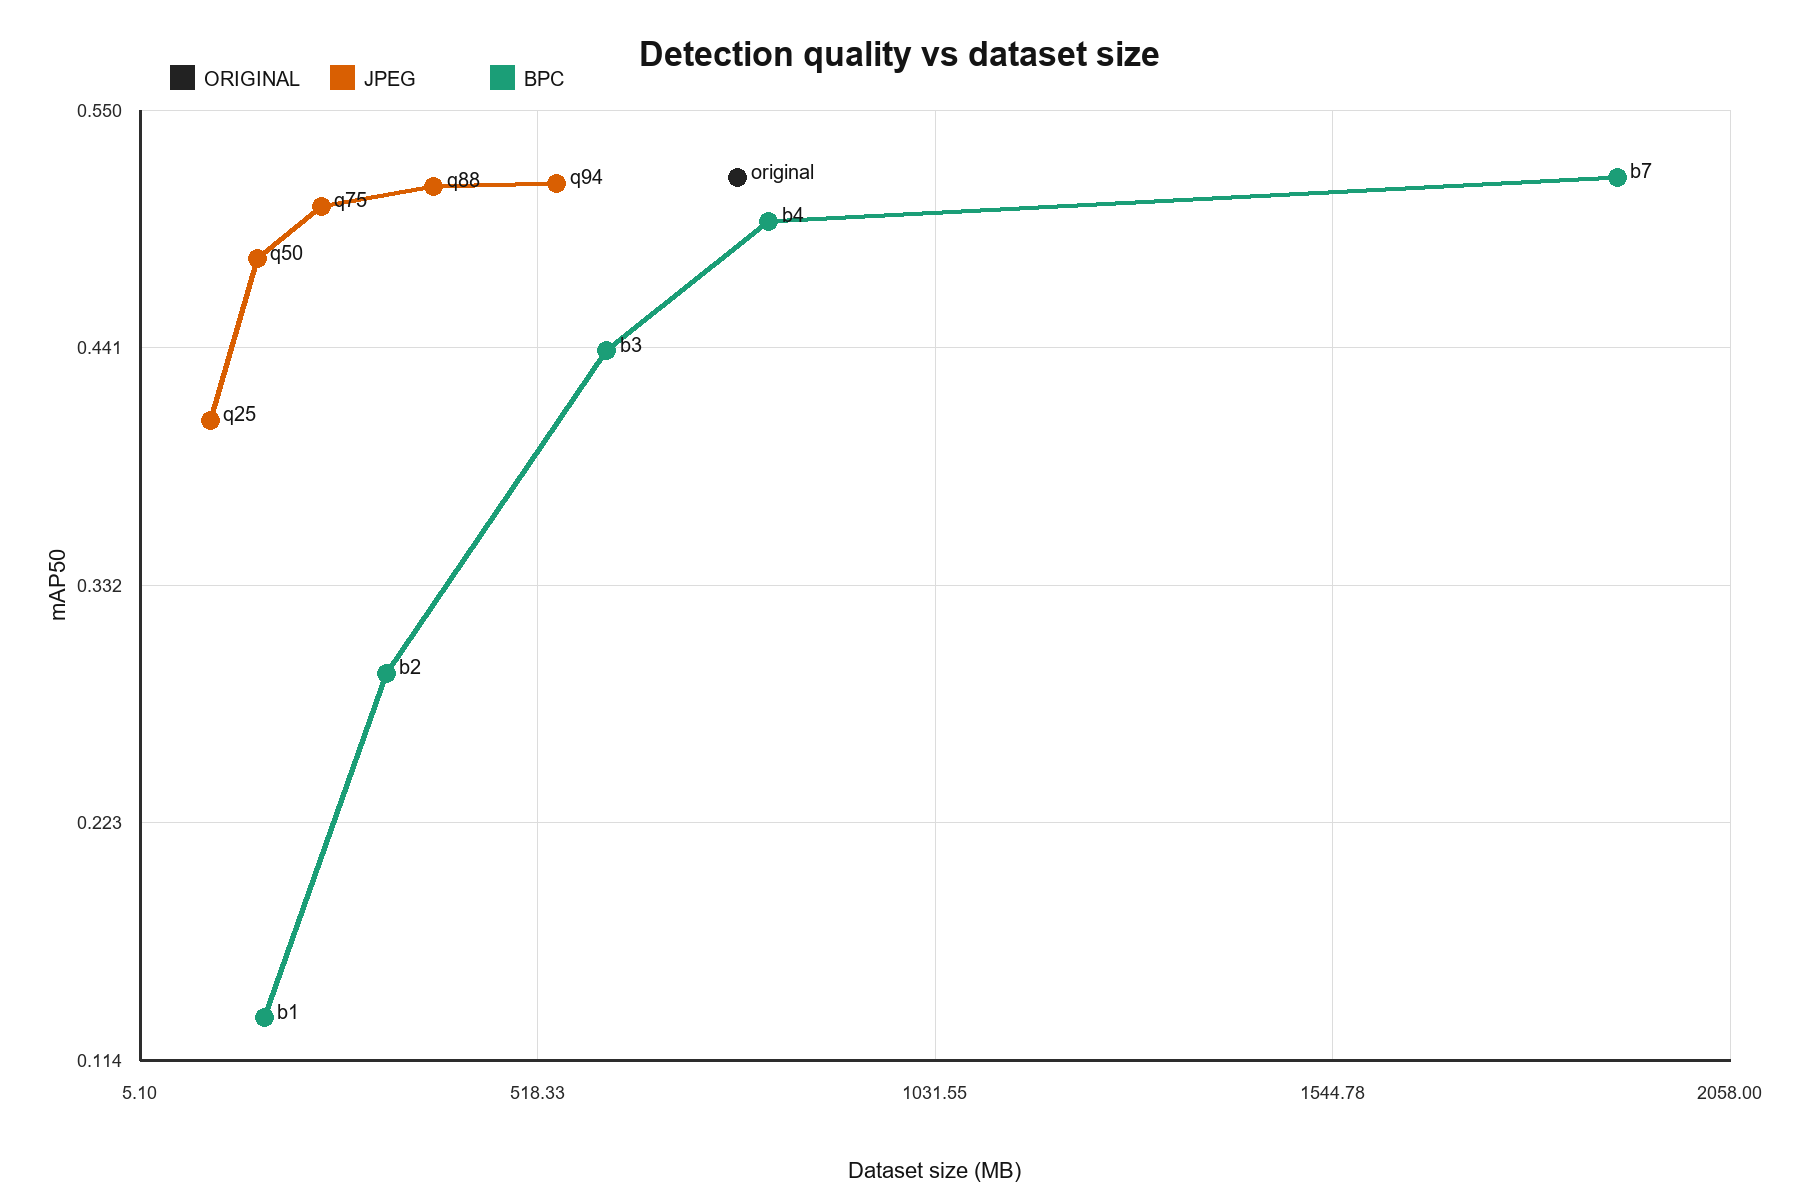
\includegraphics[width=\columnwidth]{results/article_figures/fig1_map50_vs_size.png}
\caption{Detection quality as a function of dataset size for original, JPEG, and BPC variants.}
\label{fig:map50_vs_size}
\end{figure}

As illustrated in Fig. 1, the JPEG branch displays a highly efficient, leftward curve. It aggressively reduces storage size while keeping mAP50 elevated. In contrast, the BPC branch demonstrates a disjointed path: $b7$ shifts radically to the right, doubling the baseline storage size, while modes that achieve actual size reduction ($b \le 3$) experience a vertical collapse in accuracy.

The scaling efficiency of the compression ratio against the downstream detection performance is shown in Fig. 2.

\begin{figure}[h]
\centering
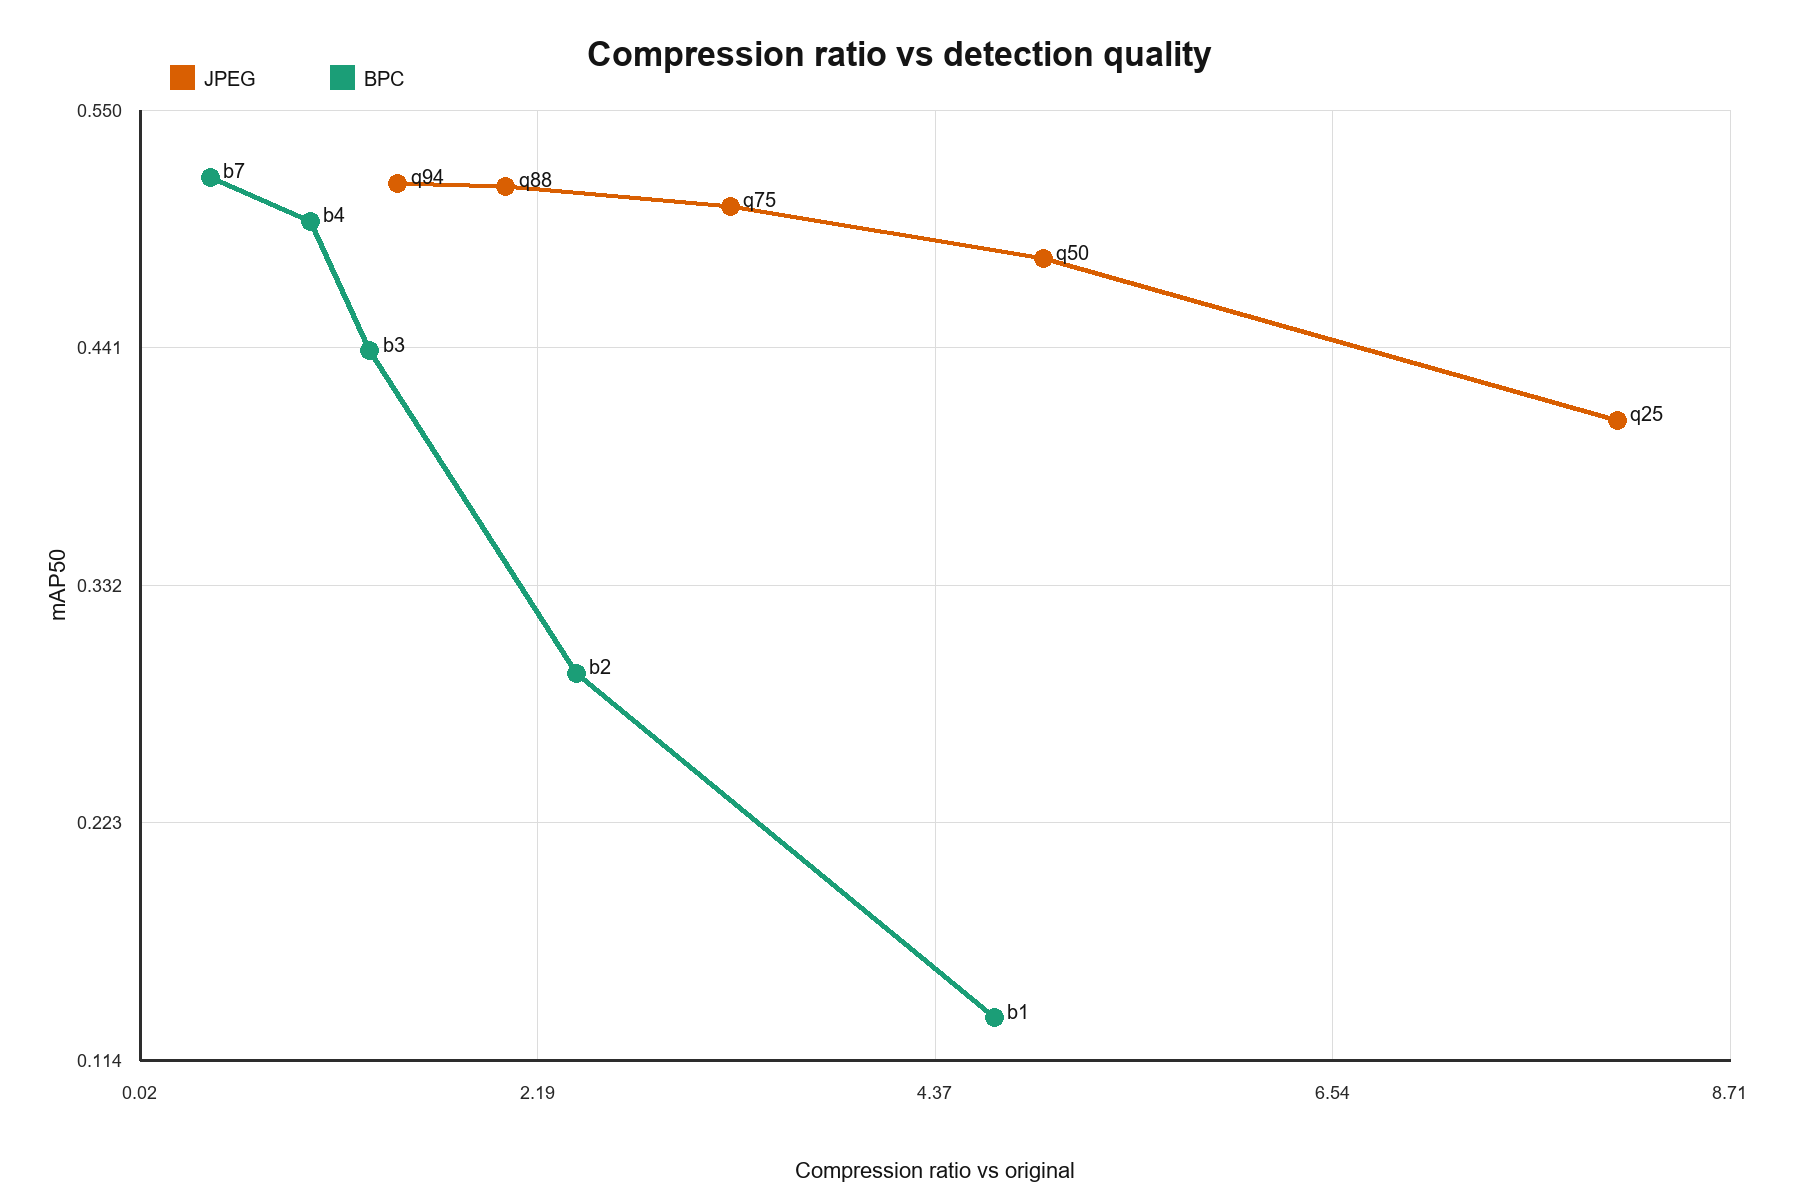
\includegraphics[width=\columnwidth]{results/article_figures/fig2_compression_ratio_vs_map50.png}
\caption{Compression ratio versus detection accuracy.}
\label{fig:cr_vs_map50}
\end{figure}

Fig. 2 highlights the dominance of JPEG in the high-compression regime. JPEG maintains a mAP50 above 0.48 up to a 5$\times$ compression factor, whereas the BPC branch drops below a 0.44 mAP50 before achieving a 1.3$\times$ compression ratio.

The relative drop in object detection performance as a function of target degradation parameters is plotted in Fig. 3.

\begin{figure}[h]
\centering
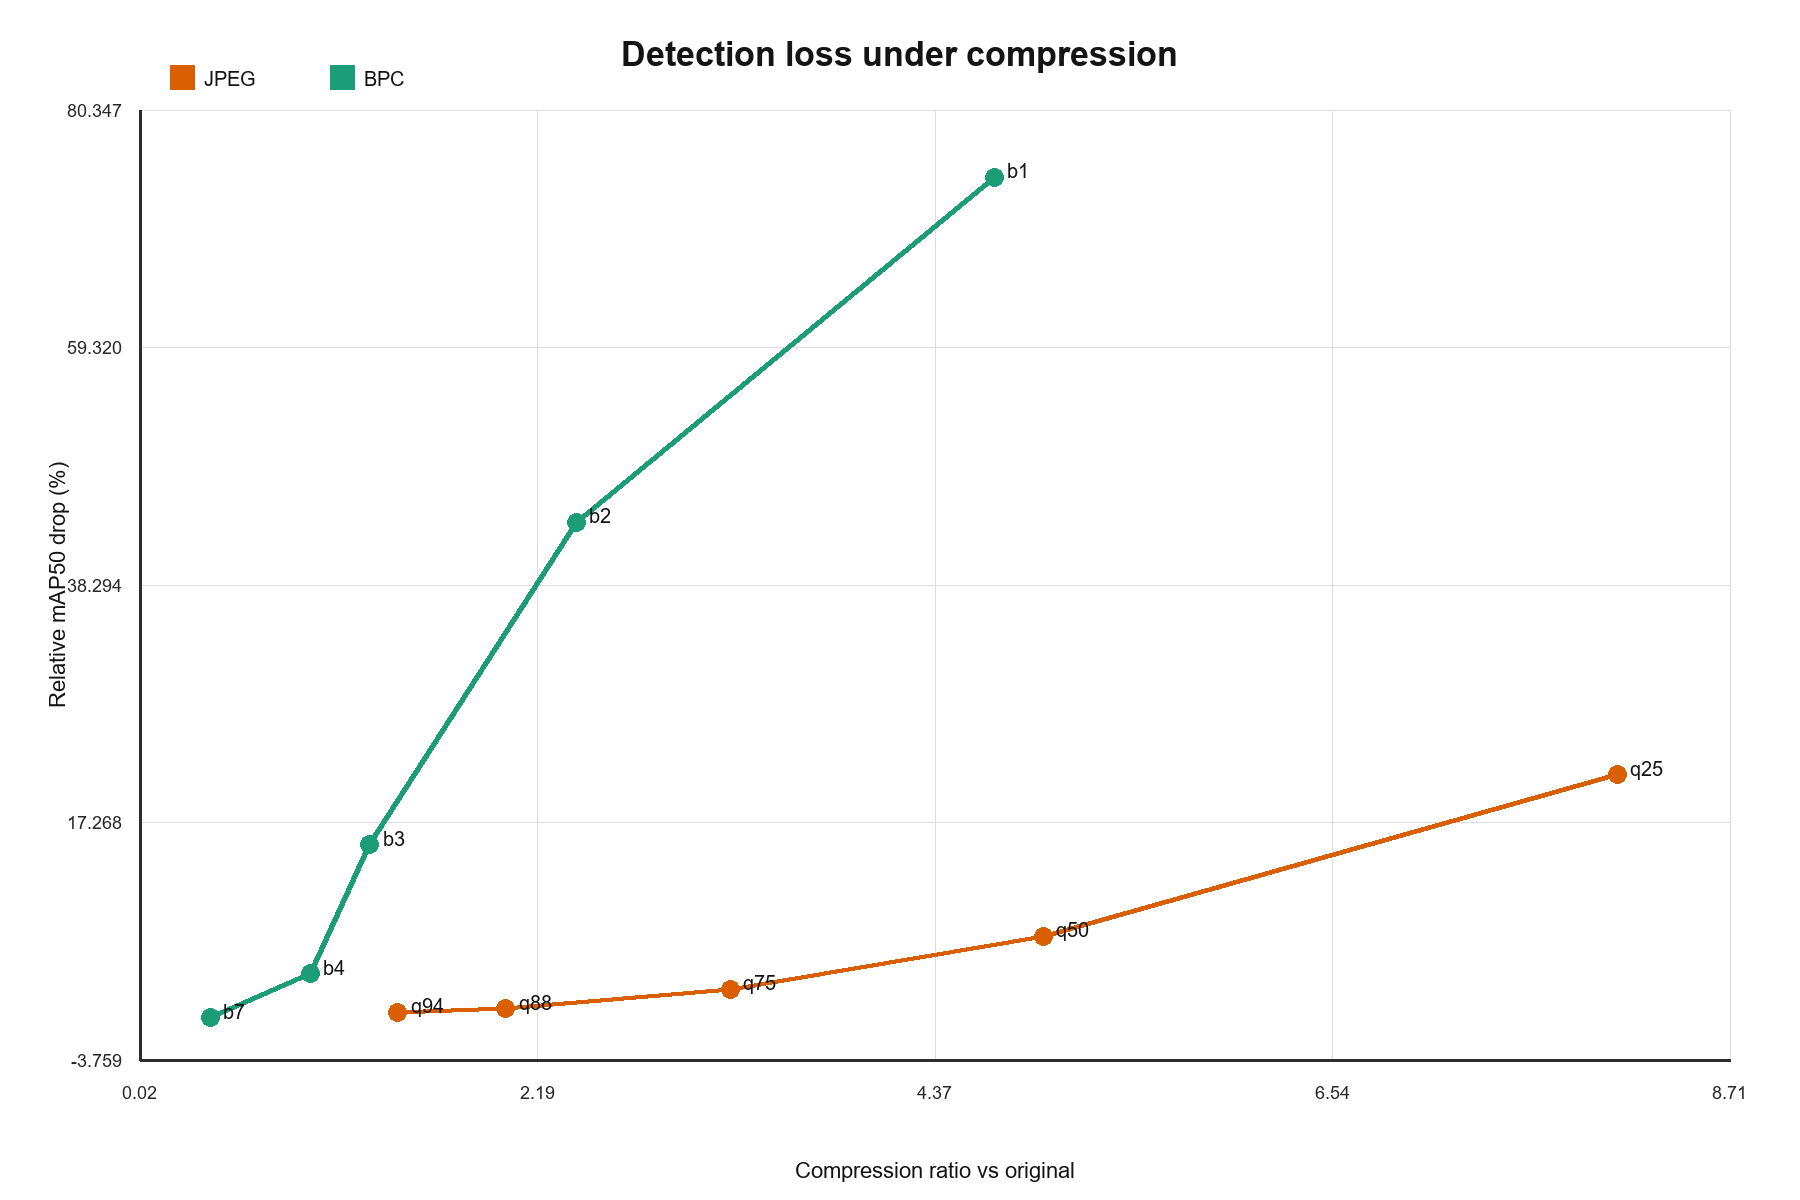
\includegraphics[width=\columnwidth]{results/article_figures/fig3_relative_map50_drop.png}
\caption{Relative mAP50 drop under different compression regimes.}
\label{fig:map50_drop}
\end{figure}

Fig. 3 illustrates that for JPEG, the accuracy drop remains below 3\% for $q \ge 75$. For BPC, the degradation is exponential: a minor drop at $b=4$ is followed by a sudden 15.3\% drop at $b=3$, and a complete failure (74.4\% relative drop) at $b=1$.

A direct comparison of the absolute physical storage footprint for each variant is provided in Fig. 4.

\begin{figure}[h]
\centering
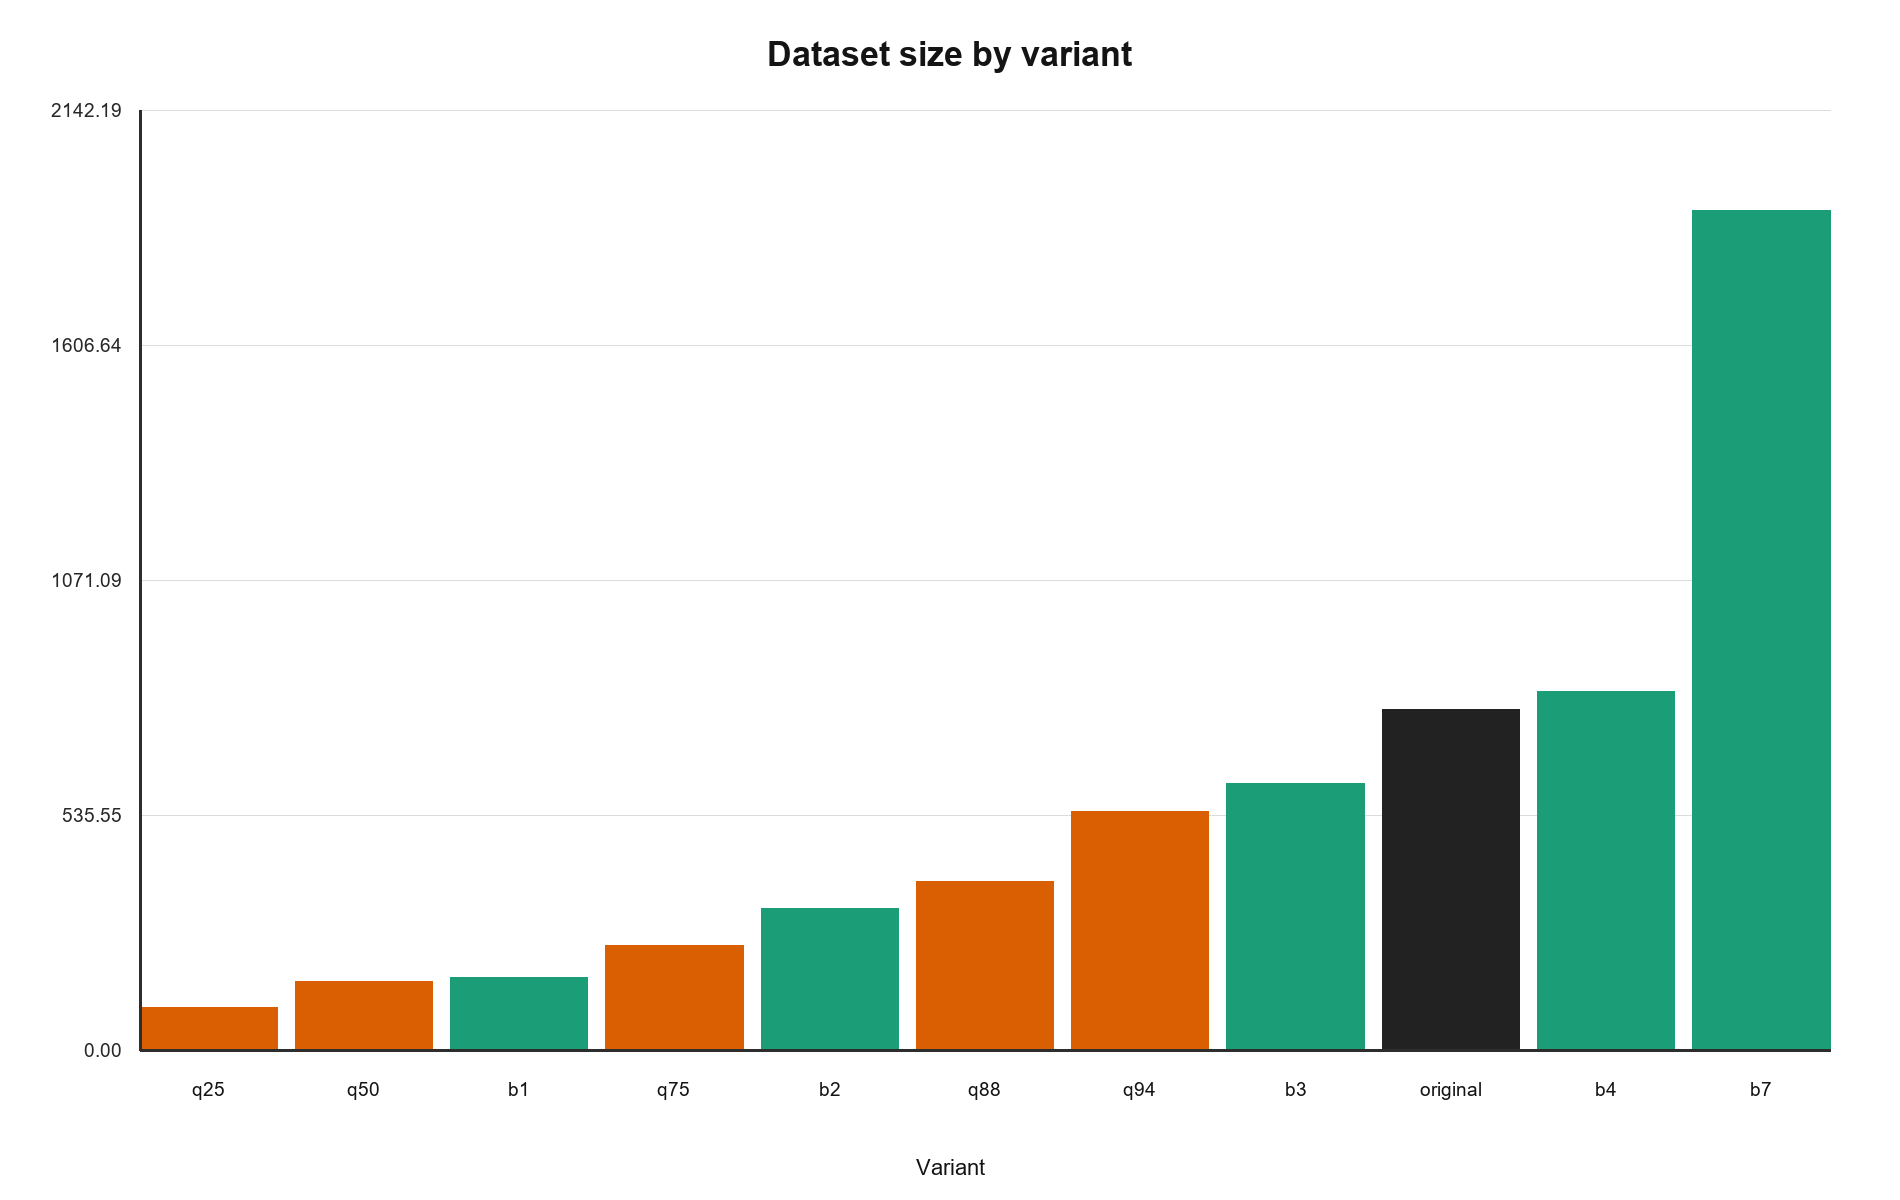
\includegraphics[width=\columnwidth]{results/article_figures/fig4_dataset_size_bars.png}
\caption{Dataset storage size compared by variant.}
\label{fig:dataset_size}
\end{figure}

Fig. 4 highlights the storage paradox of BPC: $b7$ requires an astonishing 1912.67 MB of storage---a 2.46$\times$ inflation compared to the original 776.96 MB JPEG dataset. Even $b4$ (816.80 MB) fails to yield any storage savings over the original uncompressed set.

The changes in individual object detection localization metrics (Precision and Recall) across all variants are mapped in Fig. 5.

\begin{figure}[h]
\centering
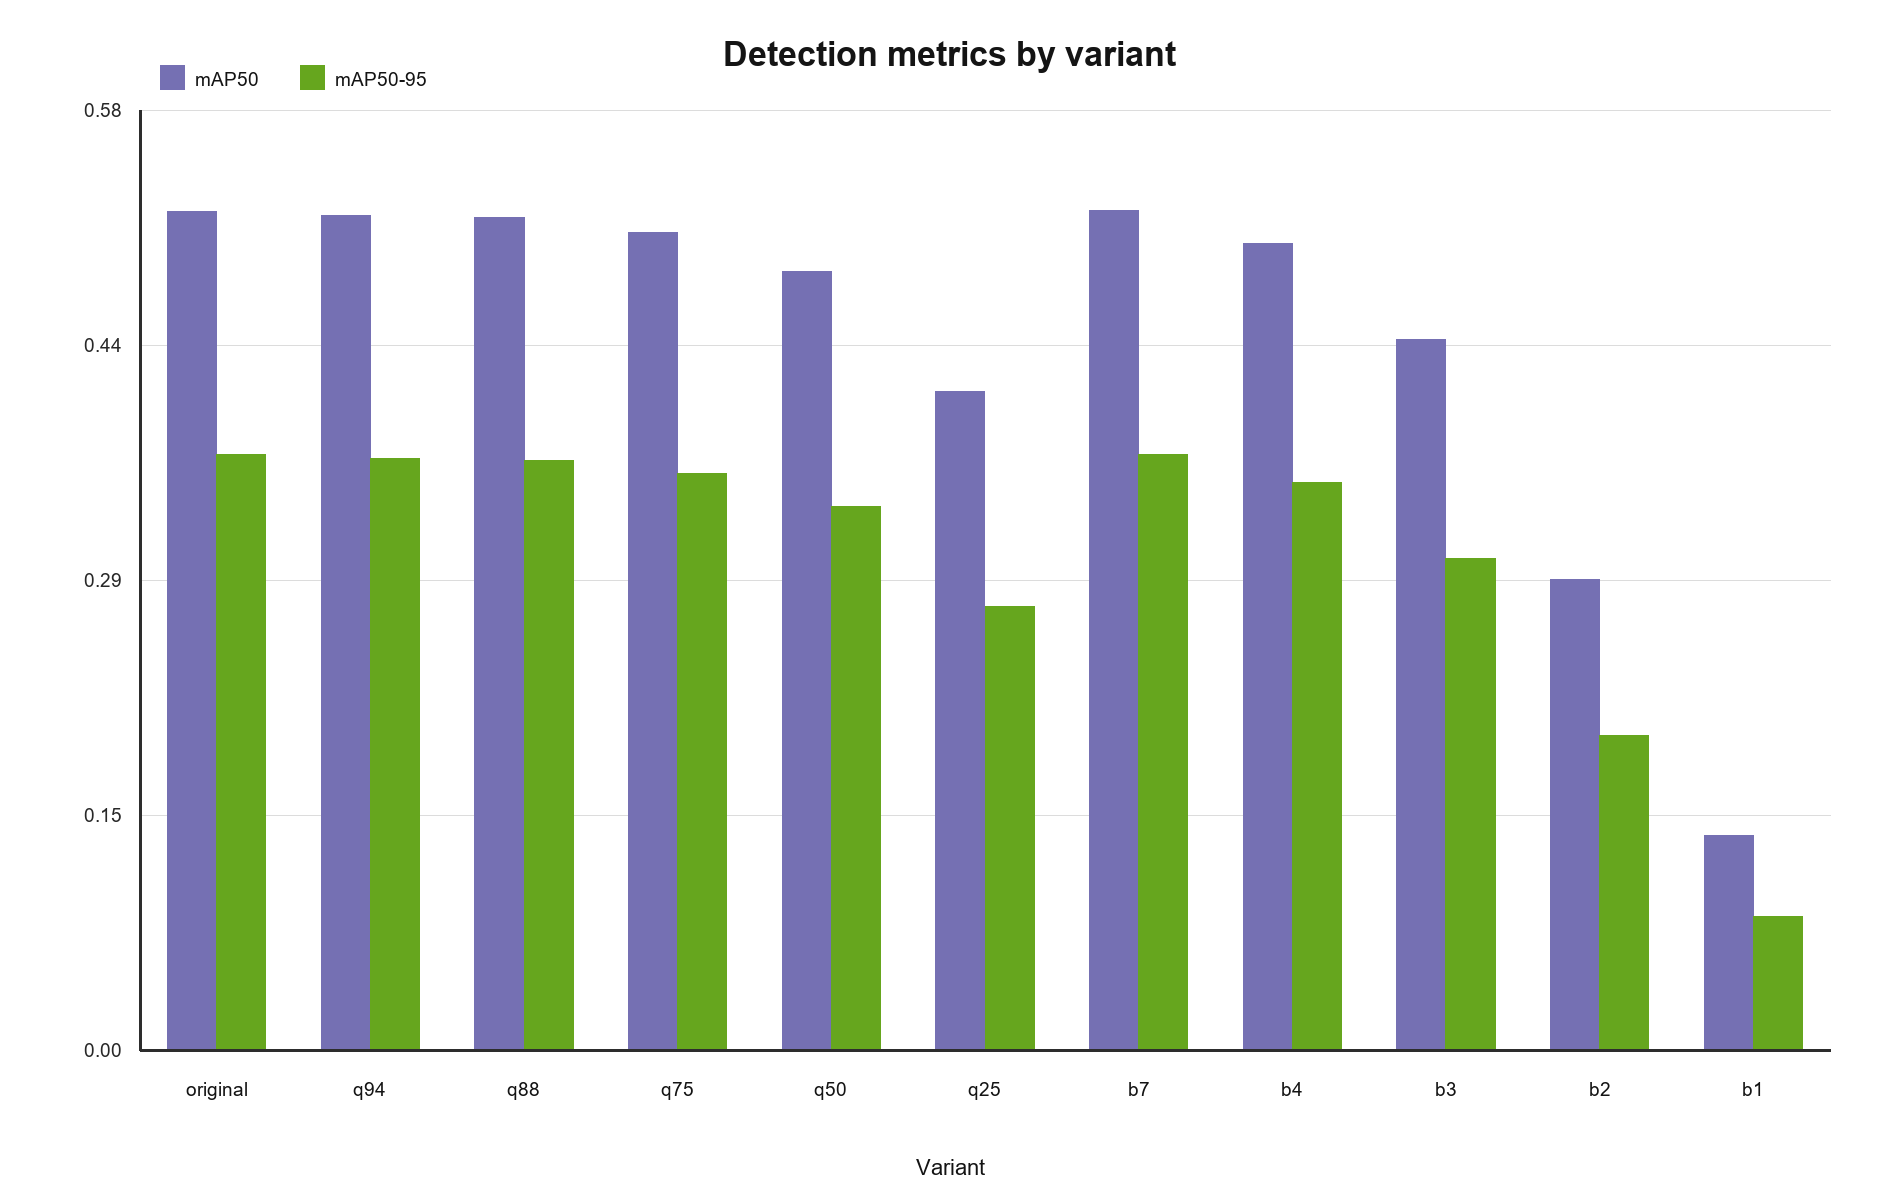
\includegraphics[width=\columnwidth]{results/article_figures/fig5_detection_metric_bars.png}
\caption{Precision and Recall trends across variants.}
\label{fig:precision_recall}
\end{figure}

Interestingly, Fig. 5 shows that for JPEG $q88$, Precision actually increases slightly to 0.6446 (from 0.6347), while Recall decreases gradually. This indicates that mild JPEG recompression acts as a high-frequency spatial filter, removing minor background textures and noise, which helps the network reduce false-positive detections.

\subsection{Divergence of Visual and Task Metrics}
The correlation between classical visual quality and downstream neural network performance is explored in Figs. 6 and 7.

The relationship between mean PSNR and downstream mAP50 is illustrated in Fig. 6.

\begin{figure}[h]
\centering
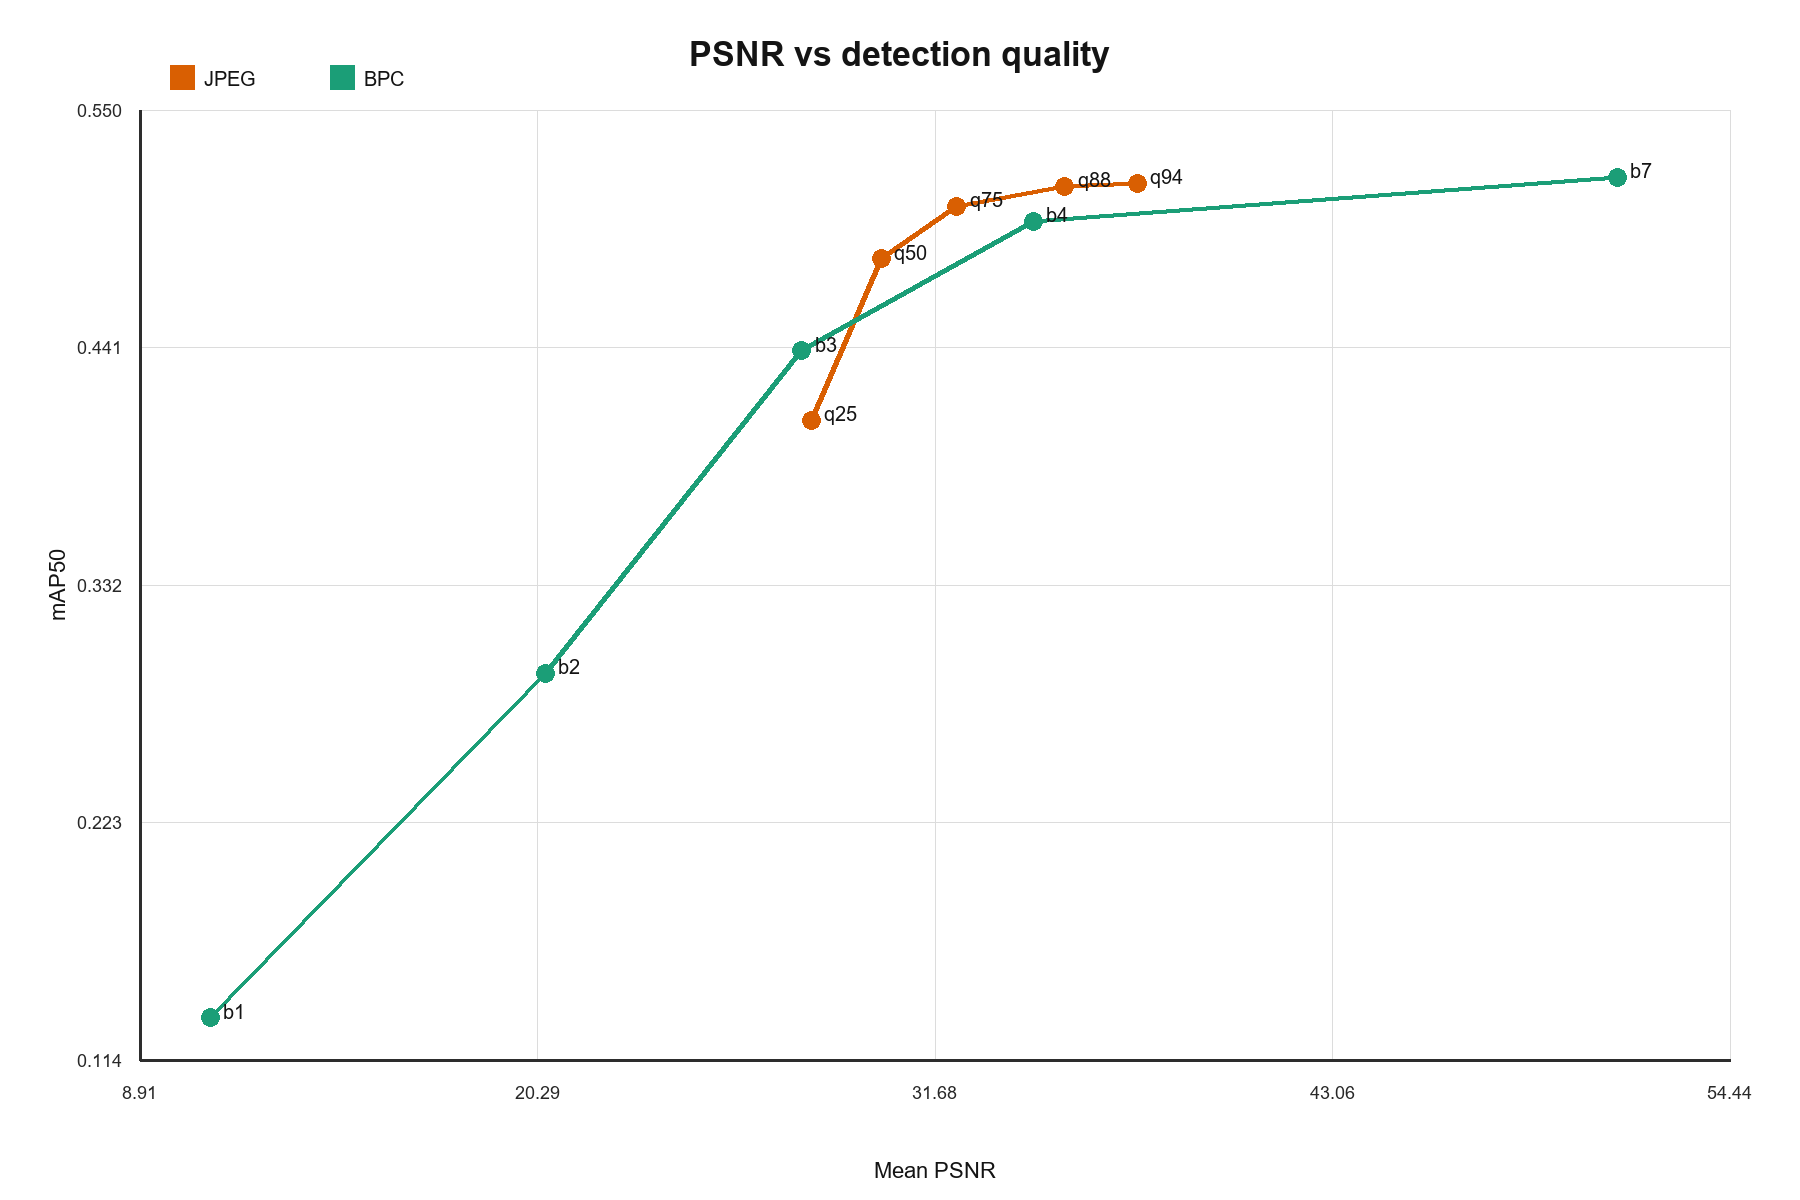
\includegraphics[width=\columnwidth]{results/article_figures/fig6_psnr_vs_map50.png}
\caption{Mean PSNR versus mAP50.}
\label{fig:psnr_vs_map50}
\end{figure}

The relationship between mean SSIM and downstream mAP50 is shown in Fig. 7.

\begin{figure}[h]
\centering
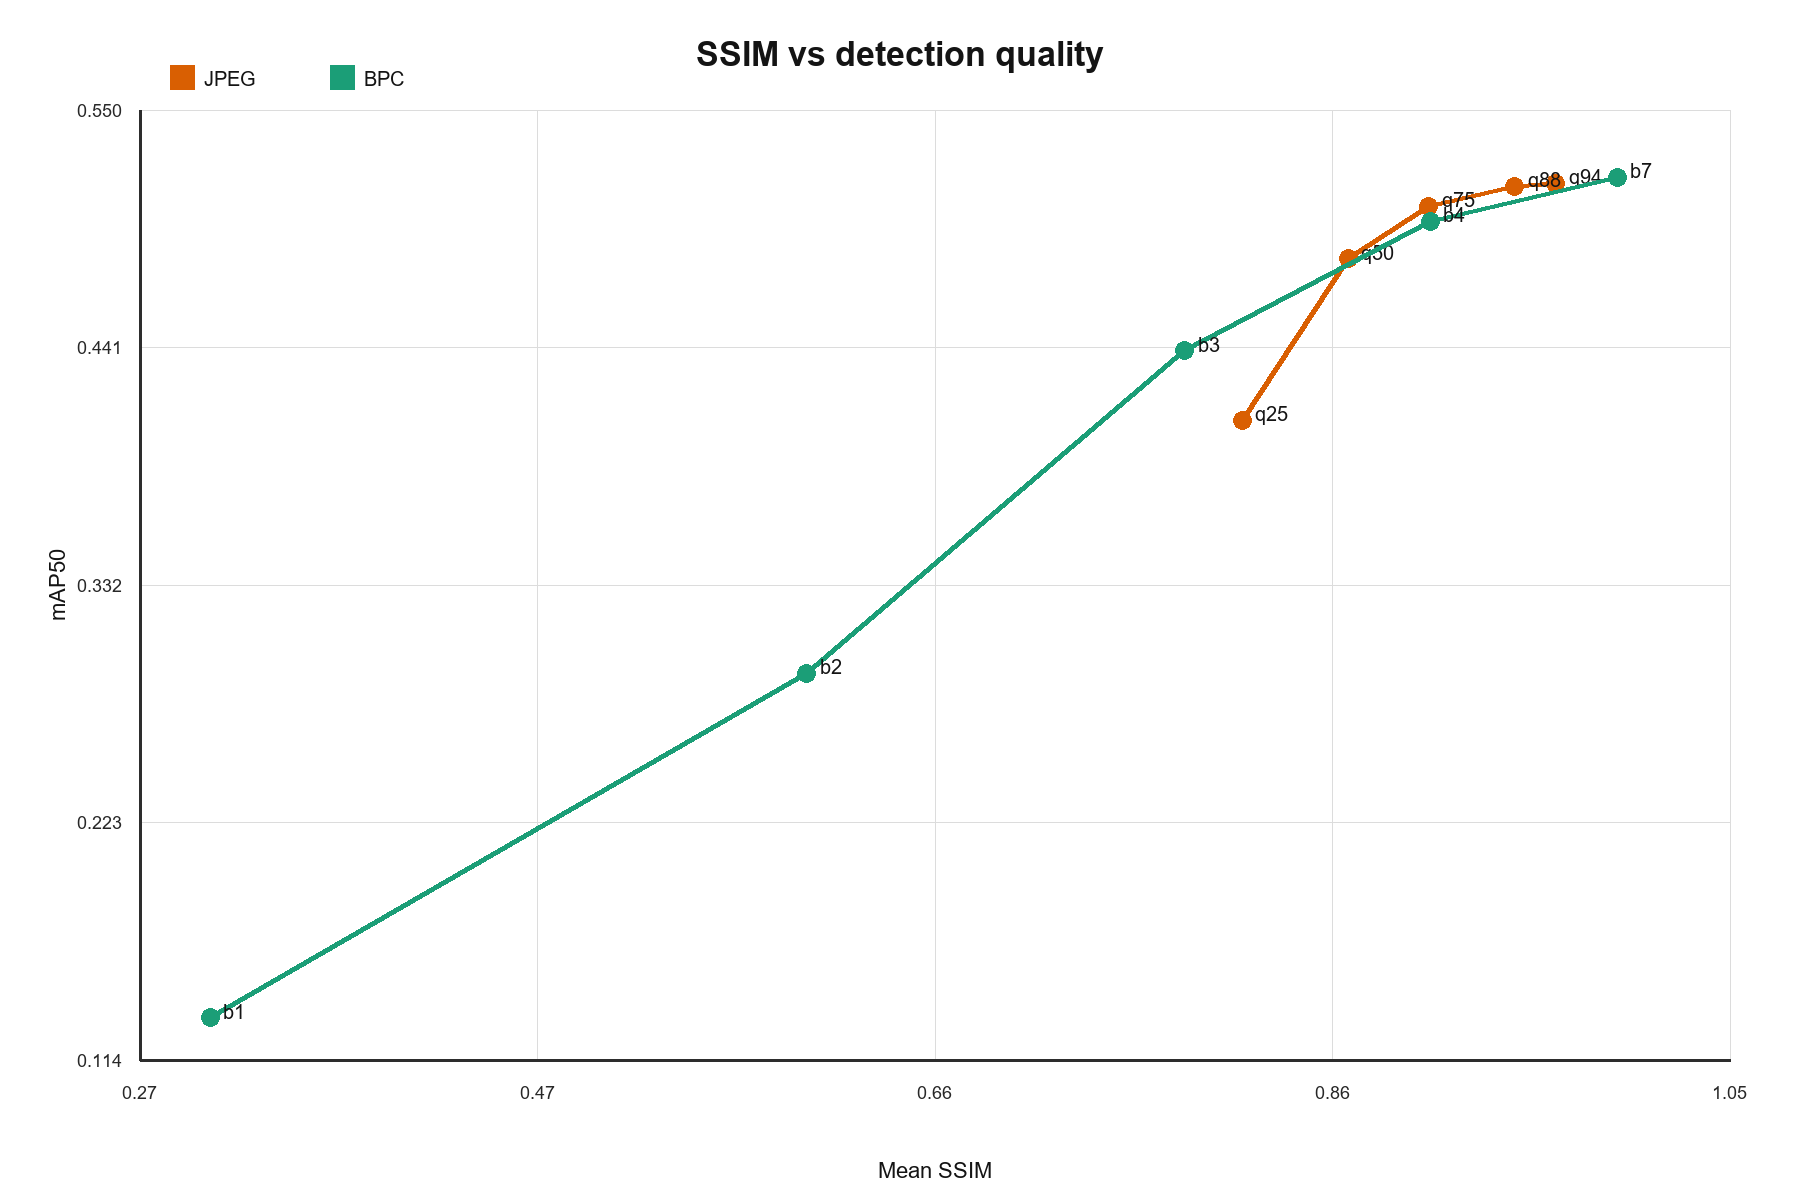
\includegraphics[width=\columnwidth]{results/article_figures/fig7_ssim_vs_map50.png}
\caption{Mean SSIM versus mAP50.}
\label{fig:ssim_vs_map50}
\end{figure}

Figs. 6 and 7 mathematically demonstrate the divergence between visual and task metrics:
\begin{itemize}
    \item \textbf{The $b7$ vs $q94$ Comparison}: $b7$ achieves a near-lossless PSNR of 51.22 dB and an SSIM of 0.9980. While it matches the baseline detection quality, it requires 3.5$\times$ more storage than $q94$ (37.47 dB PSNR, 0.9677 SSIM), which achieves the exact same object detection accuracy.
    \item \textbf{The $b4$ vs $q75$ Comparison}: $b4$ has a higher PSNR (34.48 dB vs 32.29 dB) and a higher SSIM (0.9064 vs 0.9055) than $q75$. Despite appearing visually superior, $b4$ yields a lower mAP50 (0.4987) while requiring 3.4$\times$ more storage than $q75$, which reaches a superior mAP50 of 0.5057.
\end{itemize}

\subsection{Visual Artifact Overviews}
To illustrate the visual consequences of these degradation pipelines, we examine qualitative examples of spatial structures under compression.

Examples of visual degradation for JPEG recompression across various quality factors are referenced in Fig. 8.

\begin{figure}[h]
\centering

\includegraphics[width=\columnwidth]{results/article_figures/fig8_jpeg_visual_degradation_grid.png}
\caption{Visual degradation examples for JPEG recompression (original, q88, q75, q25).}
\label{fig:jpeg_degrad}
\end{figure}

JPEG recompression (Fig. 8) exhibits high-frequency smoothing and minor blocking at $q88$ and $q75$. At $q25$, the block boundaries ($8\times8$ grids) become highly prominent, and fine textures are lost, though the coarse geometric outlines of objects remain recognizable.

Examples of visual degradation for uniform bit-depth reduction are referenced in Fig. 9.

\begin{figure}[h]
\centering

\includegraphics[width=\columnwidth]{results/article_figures/fig9_bpc_visual_degradation_grid.png}
\caption{Visual degradation examples for bit-depth reduction (original, b7, b4, b2, b1).}
\label{fig:bpc_degrad}
\end{figure}

Bit-depth reduction (Fig. 9) preserves spatial boundaries and geometric edges perfectly at $b7$ and $b4$. However, at $b4$, visible color banding (posterization) begins to appear on smooth gradients. At $b2$ and $b1$, the image disintegrates into a highly pixelated, high-contrast representation, completely destroying the smooth amplitude variations and color channels necessary for YOLOv8n's convolutional layers to register features.

\section{Discussion}
The empirical results compiled in this study provide several critical insights into the design of machine-centric digital image pipelines. Taken together, our findings substantiate the following key claims:
\begin{enumerate}
    \item Different types of image degradation affect YOLOv8 in fundamentally different ways.
    \item An equal reduction in file size does not imply equal utility of the image for object detection.
    \item A visually acceptable image is not necessarily optimal for neural network inference.
    \item Classical metrics such as PSNR and SSIM are insufficient for a complete assessment of image suitability in computer vision tasks.
    \item The choice of compression method for machine analysis must incorporate application-level detection metrics.
\end{enumerate}

\subsection{Analysis of JPEG Sweet Spots}
JPEG recompression demonstrates exceptional efficiency in the near-baseline and mid-range zones:
\begin{itemize}
    \item \textbf{The $q88$ Operating Point}: The $q88$ variant represents the strongest near-baseline trade-off identified in this research. It achieves a 2.02$\times$ compression ratio (halving the required storage footprint to 384.22 MB) with a negligible mAP50 drop of only 0.004 (0.77\% relative loss). In practical edge-AI deployments, switching the storage pipeline from raw/uncompressed JPEG to $q88$ allows systems to double their data capacity or halve transmission costs with virtually no impact on object detection accuracy.
    \item \textbf{The $q75$ Operating Point}: For systems operating under tighter storage or bandwidth constraints, $q75$ represents an outstanding compromise. It achieves 3.25$\times$ compression (reducing the dataset to 239.21 MB) while incurring a minor relative mAP50 drop of only 2.51\%.
    \item \textbf{The Role of Frequency Filtering}: The slight increase in Precision observed at $q88$ (0.6446 vs. baseline 0.6347) suggests that mild JPEG recompression acts as a beneficial spatial regularizer. By quantizing high-frequency DCT coefficients, JPEG eliminates minor pixel-level noise, dust, and microscopic background textures. This reduction in high-frequency noise prevents the YOLOv8n model from extracting false-positive features in the background, thereby boosting Precision at the cost of a minor reduction in Recall (the detection of highly obscured or distant objects).
\end{itemize}

\subsection{The BPC + PNG Storage Paradox}
The BPC branch presents a major architectural warning: \textbf{uniform bit-depth reduction stored in a standard lossless PNG container is highly inefficient for storage optimization.}
\begin{itemize}
    \item \textbf{File Size Inflation}: While 7-bit quantization ($b7$) preserves baseline detection performance perfectly (0.5189 mAP50), it inflates the dataset size to 1912.67 MB---a 146\% increase over the original baseline.
    \item \textbf{Algorithmic Explanation}: This paradox lies in how PNG handles spatial compression. Lossless PNG relies on spatial filtering (checking adjacent pixels to predict values) followed by a DEFLATE entropy encoder (which uses Huffman coding and LZ77 duplicate string matching) \cite{w3c2003}. The original COCO images are stored in a lossy, high-frequency-smoothed JPEG format. When uniform quantization is applied, the continuous, smooth color gradients of the JPEG format are broken into discrete, step-like color intervals, creating sharp, artificial boundaries (spatial banding or posterization). These high-frequency transitions act as spatial noise, causing the PNG spatial prediction filters to fail. As a result, the DEFLATE algorithm cannot find repetitive spatial strings, causing the lossless file size to inflate far beyond the original lossy JPEG baseline.
    \item \textbf{Task Collapse}: At lower bit depths ($b \le 3$), where BPC finally achieves storage savings over the original dataset (e.g., $b3$ at 607.81 MB), the color gradients are so heavily quantized that YOLOv8n experiences a severe 15.31\% mAP50 drop. At $b2$ and $b1$, the visual information collapses, leading to a catastrophic loss in object detection utility.
\end{itemize}

\subsection{Divergence of Human and Machine Quality}
Our results mathematically confirm that classical full-reference quality metrics are poor predictors of deep learning performance:
\begin{itemize}
    \item \textbf{Visual vs. Task Fidelity}: Comparing $b4$ and $q75$, we observe that $b4$ possesses a superior PSNR (34.48 dB vs. 32.29 dB) and a higher SSIM (0.9064 vs. 0.9055). To a human observer, the $b4$ image appears sharper and less distorted than the blocky $q75$ image. However, YOLOv8n achieves a superior mAP50 on $q75$ (0.5057) compared to $b4$ (0.4987), while $q75$ requires \textbf{3.4$\times$ less storage} (239.21 MB vs. 816.80 MB).
    \item \textbf{Scientific Implication}: This divergence occurs because deep convolutional neural networks extract abstract semantic features across multiple spatial hierarchies. CNNs are highly robust to the high-frequency blocky boundaries and minor color shifts introduced by JPEG recompression, but they are severely disrupted by the loss of amplitude precision and the artificial step-like color contours introduced by severe bit-depth reduction. Consequently, validating compression algorithms for automated pipelines using only PSNR/SSIM is fundamentally flawed; evaluations must incorporate task-specific downstream metrics.
\end{itemize}

The central insight that a reader should take away from this analysis is as follows: image compression cannot be evaluated for computer vision tasks using only human visual perception or PSNR/SSIM. Neural networks are sensitive to the \textit{type} of distortion, not all information loss is equally harmful, and compression for human vision and compression for machine vision are not the same problem. The choice of compression method must account for the downstream task.

\subsection{Stability and Consistency: Pilot vs. Final Results}
A crucial methodological strength of this study is the high consistency observed between our initial 500-image pilot validation (\texttt{val500}) and the final full-scale 5000-image validation (\texttt{val5k}):
\begin{itemize}
    \item \textbf{Structural Similarity of Trendlines}: The pilot experiment, conducted on Apple Silicon GPU hardware (\texttt{device=mps}), yielded the exact same structural pattern later confirmed by the single-threaded CPU \texttt{val5k} validation.
    \item \textbf{Threshold Matching}: In both the pilot and final runs, $q88$ and $q75$ emerged as the most efficient JPEG operating points. Similarly, $b7$ proved to be near-baseline in accuracy but highly inefficient in storage, while $b4$ acted as the critical threshold below which BPC performance rapidly degraded.
    \item \textbf{Scientific Confidence}: The replication of these complex non-linear curves across different subset sizes and hardware execution targets significantly strengthens the scientific confidence in our findings, demonstrating that our task-aware analysis represents a highly stable and generalizable empirical trend.
\end{itemize}

\section{Conclusion}
This study presents a rigorous task-aware evaluation of image compression and quantization strategies, demonstrating that the visual appeal of an image to a human observer does not predict its utility for automated deep learning systems.

\subsection{Main Findings}
Under the evaluated conditions, the following key propositions are empirically established:
\begin{enumerate}
    \item The effectiveness of image compression for object detection tasks must be evaluated not only by visual quality metrics but also by downstream task metrics.
    \item JPEG compression and bit-depth reduction at comparable compression levels exert fundamentally different effects on object detection quality.
    \item The nature of the distortions introduced is no less important a factor than the overall level of information loss.
    \item Moderate bit-depth reduction can preserve task-relevant information; however, the practical efficiency of this approach depends critically on the storage format.
    \item For practical computer vision systems, the optimal compression method must be selected based on the trade-off between data volume and model performance on the downstream task.
\end{enumerate}

Specifically, JPEG quality factor \textbf{q88} represents the most efficient practical operating point, halving the dataset storage size (2.02$\times$ compression) with less than a 1\% relative drop in object detection accuracy ($mAP50 = 0.5147$ vs. baseline $0.5187$). For tighter budgets, \textbf{q75} provides 3.25$\times$ compression with only a 2.51\% mAP50 drop. Uniform RGB bit-depth reduction stored in PNG is highly inefficient: it introduces spatial banding that disrupts the PNG DEFLATE compressor, causing file size inflation at high bit depths ($b7$ is 2.46$\times$ larger than baseline) and collapsing downstream detection accuracy at lower bit depths. Traditional visual quality metrics (PSNR, SSIM) diverge significantly from neural network task metrics (mAP), confirming that human-centric evaluation is insufficient for machine vision engineering.

Although moderate bit-depth reduction preserves information that is meaningful for YOLOv8, under the evaluated data representation scheme it is inferior to JPEG recompression in terms of the combined storage size and detection quality trade-off. This is a legitimate and valuable scientific result: the study demonstrates that it is not simply the quantity of lost information that matters, but rather what kind of information is lost.

\subsection{Limitations of the Study}
We acknowledge several key boundaries of our current experimental scope:
\begin{itemize}
    \item \textbf{Detector Architecture}: Our evaluations were restricted to a single real-time detector family (YOLOv8n).
    \item \textbf{Dataset Diversity}: The empirical trends were evaluated solely on the Microsoft COCO val2017 dataset.
    \item \textbf{BPC Storage Scope}: The bit-depth reduction branch was restricted to uniform RGB quantization saved via a standard lossless PNG container.
    \item \textbf{Recompression Nature}: The JPEG branch evaluated represents second-order lossy recompression, as the original COCO source images were already stored in JPEG format.
    \item \textbf{Hardware Platform}: The final validation was conducted on a single-threaded CPU environment. The conclusions pertain to the tested setup and require careful generalization.
\end{itemize}

\subsection{Future Work}
To expand this research into a comprehensive framework, future investigations will focus on the following areas:
\begin{enumerate}
    \item \textbf{Advanced Codec Evaluations}: Evaluating modern lossy and lossless codecs, including WebP, AVIF, and JPEG XL, to identify if newer spatial and frequency transforms yield superior task-aware compression profiles.
    \item \textbf{Alternative Detector Families}: Testing the generalizability of these findings across different detector paradigms, such as two-stage detectors (Faster R-CNN), anchor-based models (YOLOv5), and vision-transformer-based detectors (DETR).
    \item \textbf{Learned Machine-Centric Compression}: Integrating end-to-end learned image compression networks trained directly with a joint loss function combining rate-distortion optimization and downstream detection loss.
    \item \textbf{Statistical Stability and Per-Class Analysis}: Conducting repeated statistical runs with varied initial seeds, alongside a per-class detection analysis to identify if specific semantic categories (e.g., small objects vs. large structures) display unique sensitivities to frequency-domain or amplitude-domain quantization noise.
    \item \textbf{Entropy Coding for Low Bit-Depths}: Exploring customized, spatial-aware entropy encoders for quantized bit-depth images that bypass the limitations of the PNG container, enabling real storage savings for low-bit-depth machine vision inputs.
\end{enumerate}

\begin{thebibliography}{20}

\bibitem{wallace1992}
Wallace, G. K. (1992). The JPEG still picture compression standard. \textit{IEEE Transactions on Consumer Electronics}, \textit{38}(1), xviii–xxxiv. https://doi.org/10.1109/30.125072

\bibitem{w3c2003}
World Wide Web Consortium. (2003). \textit{Portable Network Graphics (PNG) specification (second edition)} (W3C Recommendation 10 November 2003). https://www.w3.org/TR/PNG/

\bibitem{wang2004}
Wang, Z., Bovik, A. C., Sheikh, H. R., \& Simoncelli, E. P. (2004). Image quality assessment: From error visibility to structural similarity. \textit{IEEE Transactions on Image Processing}, \textit{13}(4), 600–612. https://doi.org/10.1109/TIP.2003.819861

\bibitem{hore2010}
Horé, A., \& Ziou, D. (2010). Image quality metrics: PSNR vs. SSIM. \textit{2010 20th International Conference on Pattern Recognition}, 2366–2369. https://doi.org/10.1109/ICPR.2010.579

\bibitem{zhai2020}
Zhai, G., \& Min, X. (2020). Perceptual image quality assessment: A survey. \textit{Science China Information Sciences}, \textit{63}(11), 211301. https://doi.org/10.1007/s11432-019-2757-1

\bibitem{jocher2023}
Jocher, G., Chaurasia, A., \& Qiu, J. (2023). \textit{Ultralytics YOLOv8} (Version 8.0.0) [Computer software]. https://github.com/ultralytics/ultralytics

\bibitem{redmon2016}
Redmon, J., Divvala, S., Girshick, R., \& Farhadi, A. (2016). You only look once: Unified, real-time object detection. \textit{Proceedings of the IEEE Conference on Computer Vision and Pattern Recognition (CVPR)}, 779–788. https://doi.org/10.1109/CVPR.2016.91

\bibitem{wang2023}
Wang, C.-Y., Bochkovskiy, A., \& Liao, H.-Y. M. (2023). YOLOv7: Trainable bag-of-freebies sets new state-of-the-art for real-time object detectors. \textit{Proceedings of the IEEE/CVF Conference on Computer Vision and Pattern Recognition (CVPR)}, 7464–7475. https://doi.org/10.1109/CVPR52729.2023.00721

\bibitem{lin2014}
Lin, T.-Y., Maire, M., Belongie, S. J., Hays, J., Perona, P., Ramanan, D., Dollár, P., \& Zitnick, C. L. (2014). Microsoft COCO: Common objects in context. In D. Fleet, T. Pajdla, B. Schiele, \& T. Tuytelaars (Eds.), \textit{Computer vision – ECCV 2014} (pp. 740–755). Springer. https://doi.org/10.1007/978-3-319-10602-1\_48

\bibitem{hu2018}
Hu, Y., Yang, W., Li, J., \& Wang, L. (2018). Content-aware and task-aware image compression for cloud-based object detection. \textit{Proceedings of the IEEE/CVF Conference on Computer Vision and Pattern Recognition (CVPR) Workshops}, 1689–1697. https://doi.org/10.1109/CVPRW.2018.00220

\bibitem{kim2021}
Kim, M., Lee, J., \& Kim, C. (2021). Task-aware image compression via spatially-adaptive feature transform. \textit{arXiv preprint arXiv:2108.09551}. https://arxiv.org/abs/2108.09551

\bibitem{ye2023}
Ye, J., Yeo, H., Park, J., \& Han, D. (2023). AccelIR: Task-aware image compression for accelerating neural restoration. \textit{Proceedings of the IEEE/CVF Conference on Computer Vision and Pattern Recognition (CVPR)}, 17852–17861. https://doi.org/10.1109/CVPR.2023.01712

\bibitem{gandor2022}
Gandor, T., \& Nalepa, J. (2022). First gradually, then suddenly: Understanding the impact of image compression on object detection using deep learning. \textit{Sensors}, \textit{22}(3), 1104. https://doi.org/10.3390/s22031104

\bibitem{hao2022}
Hao, Y., Pei, H., Lyu, Y., Yuan, Z., Rizzo, J.-R., Wang, Y., \& Fang, Y. (2022). \textit{Understanding the impact of image quality and distance of objects to object detection performance}. arXiv preprint arXiv:2209.08237. https://doi.org/10.48550/arXiv.2209.08237

\bibitem{huang2024}
Huang, C.-H., \& Wu, J.-L. (2024). Unveiling the future of human and machine coding: A survey of end-to-end learned image compression. \textit{Entropy}, \textit{26}(5), 357. https://doi.org/10.3390/e26050357

\bibitem{piran2022}
Piran, M. J. (2022). Learning-driven lossy image compression: A comprehensive survey. \textit{arXiv preprint arXiv:2201.09240}. https://doi.org/10.48550/arXiv.2201.09240

\bibitem{heckbert1982}
Heckbert, P. S. (1982). Color image quantization for frame buffer display. \textit{Proceedings of the 9th Annual Conference on Computer Graphics and Interactive Techniques (SIGGRAPH ’82)}, 297–307. https://doi.org/10.1145/800064.801294

\bibitem{floyd1976}
Floyd, R. W., \& Steinberg, L. (1976). An adaptive algorithm for spatial grey scale. \textit{Proceedings of the Society of Information Display}, \textit{17}(2), 75–77.

\bibitem{jacob2018}
Jacob, B., Kligys, S., Chen, B., Zhu, M., Tang, M., Howard, A., Adam, H., \& Kalenichenko, D. (2018). Quantization and training of neural networks for efficient integer-arithmetic-only inference. \textit{Proceedings of the IEEE Conference on Computer Vision and Pattern Recognition (CVPR)}, 2704–2713. https://doi.org/10.1109/CVPR.2018.00291

\bibitem{han2016}
Han, S., Mao, H., \& Dally, W. J. (2016). Deep compression: Compressing deep neural networks with pruning, trained quantization and Huffman coding. \textit{International Conference on Learning Representations (ICLR)}. https://arxiv.org/abs/1510.00149

\end{thebibliography}

\end{document}